\section{Homotopy groups from the Hopf bundles}\label{ch:groups}

\subsection{The splitting}

\begin{proof}[Proof of Theorem~\ref{thm:C}]
Let $d\in\{2,4,8\}$ and let $F=h_\K^{-1}(N_0)=\{(a,0):|a|=1\}\cong S^{d-1}$ be the fibre over the north pole. By Corollary~\ref{cor:fibration}, $h_\K$ is a fibration. The inclusion $j\colon F\to S^{2d-1}$ is null-homotopic, because $\pi_{d-1}(S^{2d-1})=0$ by Proposition~\ref{prop:below}; explicitly,
\begin{equation}\label{eq:nullhomotopy}
G\colon F\times[0,\tfrac\pi2]\to S^{2d-1},\qquad G(a,s)=(a\cos s,\;\sin s)
\end{equation}
contracts $F$ to the point $(0,1)$. All three spaces are path connected, and $\pi_{i-1}(S^{d-1})$ is abelian for $i\ge2$ (it is $\pi_1(S^1)\cong\Z$ or zero when $i=2$). Lemma~\ref{lem:split} gives the split exact sequence
\[
0\to\pi_i(S^{2d-1})\xrightarrow{(h_\K)_*}\pi_i(S^d)\xrightarrow{\ \partial\ }\pi_{i-1}(S^{d-1})\to0 .
\]
For $d=2$ and $i\ge3$ the third group is $\pi_{i-1}(S^1)=0$ by Example~\ref{ex:covering}, so $(h_\C)_*$ is an isomorphism. The values $\pi_6(S^3)\cong\Z/12$, $\pi_7(S^3)\cong\Z/2$ and $\pi_{14}(S^7)\cong\Z/120$ are taken from Toda's tables (I6), \cite[Chapter~XIV]{Tod62}, and give $\pi_7(S^4)\cong\Z\oplus\Z/12$, $\pi_8(S^4)\cong(\Z/2)^2$ and $\pi_{15}(S^8)\cong\Z\oplus\Z/120$. The infinite cyclic summand of $\pi_{2d-1}(S^d)$ is $(h_\K)_*\pi_{2d-1}(S^{2d-1})$, generated by $[h_\K]$, and by Proposition~\ref{prop:composition} the Hopf invariant of $(h_\K)_*[g]=[h_\K\circ g]$ is $\pm\deg g$; so it detects this summand.
\end{proof}

The splitting map of Lemma~\ref{lem:split} can be identified.

\begin{proposition}\label{prop:sigmaE}
For the null-homotopy \eqref{eq:nullhomotopy}, the splitting $\sigma\colon\pi_{i-1}(S^{d-1})\to\pi_i(S^d)$ of \eqref{eq:sigma} is the suspension homomorphism $E$, up to a sign that depends only on orientation conventions. Hence
\[
\pi_i(S^d)=(h_\K)_*\pi_i(S^{2d-1})\;\oplus\;E\,\pi_{i-1}(S^{d-1})\qquad(d=2,4,8,\ i\ge2),
\]
and the suspensions $E\colon\pi_{i-1}(S^3)\to\pi_i(S^4)$ and $E\colon\pi_{i-1}(S^7)\to\pi_i(S^8)$ are injective for every $i$.
\end{proposition}

\begin{proof}
Composing $G$ with $h_\K$ gives
\[
h_\K\bigl(G(a,s)\bigr)=\bigl(2a\cos s\sin s,\;\cos^2s-\sin^2s\bigr)=\bigl(a\sin2s,\;\cos2s\bigr),
\]
which, as $s$ runs from $0$ to $\pi/2$, moves the point $a$ of the fibre along the meridian of $S^d$ from the north pole through the direction $a$ to the south pole. For $\beta\colon S^{i-2}\to F$, the element $\sigma[\beta]$ is represented by $(u,s)\mapsto(\beta(u)\sin2s,\cos2s)$ on $S^{i-2}\times[0,\pi/2]$, which collapses $S^{i-2}\times\{0\}$ to the north pole and $S^{i-2}\times\{\pi/2\}$ to the south pole. This is the unreduced suspension of $\beta$ followed by the identification $\Sigma S^{d-1}\cong S^d$ given by meridians; as an element of $\pi_i(S^d)$ it is $\pm E[\beta]$, the unreduced and reduced suspensions being homotopy equivalent. The last statement holds because $\sigma=\pm E$ is a split injection.
\end{proof}

\begin{remark}
For $d=2$ and $i=2$ the proposition gives $\pi_2(S^2)=E\pi_1(S^1)\cong\Z$, generated by $E[\mathrm{id}_{S^1}]=[\mathrm{id}_{S^2}]$, in accordance with Proposition~\ref{prop:degree}. For $d=4$ it recovers the classical decomposition $\pi_i(S^4)\cong\pi_i(S^7)\oplus\pi_{i-1}(S^3)$ with the second summand embedded by suspension \cite[Chapter~V]{Tod62}.
\end{remark}

\subsection{The table of unstable groups}\label{sec:table}

Table~\ref{tab:unstable} lists $\pi_{n+k}(S^n)$ for $k\le7$ and $n\le9$, with the stable value in the last column. All entries are taken from Toda \cite{Tod62}, but the entries in the columns $n=2,4,8$ are also consequences of Theorem~\ref{thm:C} and the entries in the columns $n=3$, $n=7$; the columns $n\ge k+2$ are constant by Freudenthal's theorem. Figure~\ref{fig:table} shows the same table with the three kinds of entries distinguished. That the table is consistent with Theorem~\ref{thm:C} and with Theorem~\ref{thm:freudenthal}, as abelian groups, is checked by the program of Appendix~\ref{app:checks}.

\begin{table}[ht]
\centering
\small
\setlength{\tabcolsep}{4.2pt}
\begin{tabular}{@{}c|ccccccccc|c@{}}
\toprule
$k\backslash n$ & $1$ & $2$ & $3$ & $4$ & $5$ & $6$ & $7$ & $8$ & $9$ & $\pi_k^s$\\
\midrule
$0$ & $\Z$ & $\Z$ & $\Z$ & $\Z$ & $\Z$ & $\Z$ & $\Z$ & $\Z$ & $\Z$ & $\Z$\\
$1$ & $0$ & $\Z$ & $2$ & $2$ & $2$ & $2$ & $2$ & $2$ & $2$ & $2$\\
$2$ & $0$ & $2$ & $2$ & $2$ & $2$ & $2$ & $2$ & $2$ & $2$ & $2$\\
$3$ & $0$ & $2$ & $12$ & $\Z{\oplus}12$ & $24$ & $24$ & $24$ & $24$ & $24$ & $24$\\
$4$ & $0$ & $12$ & $2$ & $2^2$ & $2$ & $0$ & $0$ & $0$ & $0$ & $0$\\
$5$ & $0$ & $2$ & $2$ & $2^2$ & $2$ & $\Z$ & $0$ & $0$ & $0$ & $0$\\
$6$ & $0$ & $2$ & $3$ & $24{\oplus}3$ & $2$ & $2$ & $2$ & $2$ & $2$ & $2$\\
$7$ & $0$ & $3$ & $15$ & $15$ & $30$ & $60$ & $120$ & $\Z{\oplus}120$ & $240$ & $240$\\
\bottomrule
\end{tabular}
\caption{The groups $\pi_{n+k}(S^n)$ for $0\le k\le7$, after Toda \cite{Tod62}; an integer $m$ stands for $\Z/m$ and $2^2$ for $(\Z/2)^2$. The column $n=2$ equals the column $n=3$ shifted down by one row; the column $n=4$ is the sum of the column $n=7$ shifted down by three rows and the column $n=3$; the column $n=8$ is the sum of the column $n=7$ and the group $\pi_{8+k}(S^{15})$, which is $\Z$ for $k=7$ and $0$ for $k<7$.}
\label{tab:unstable}
\end{table}

\begin{figure}[ht]
\centering
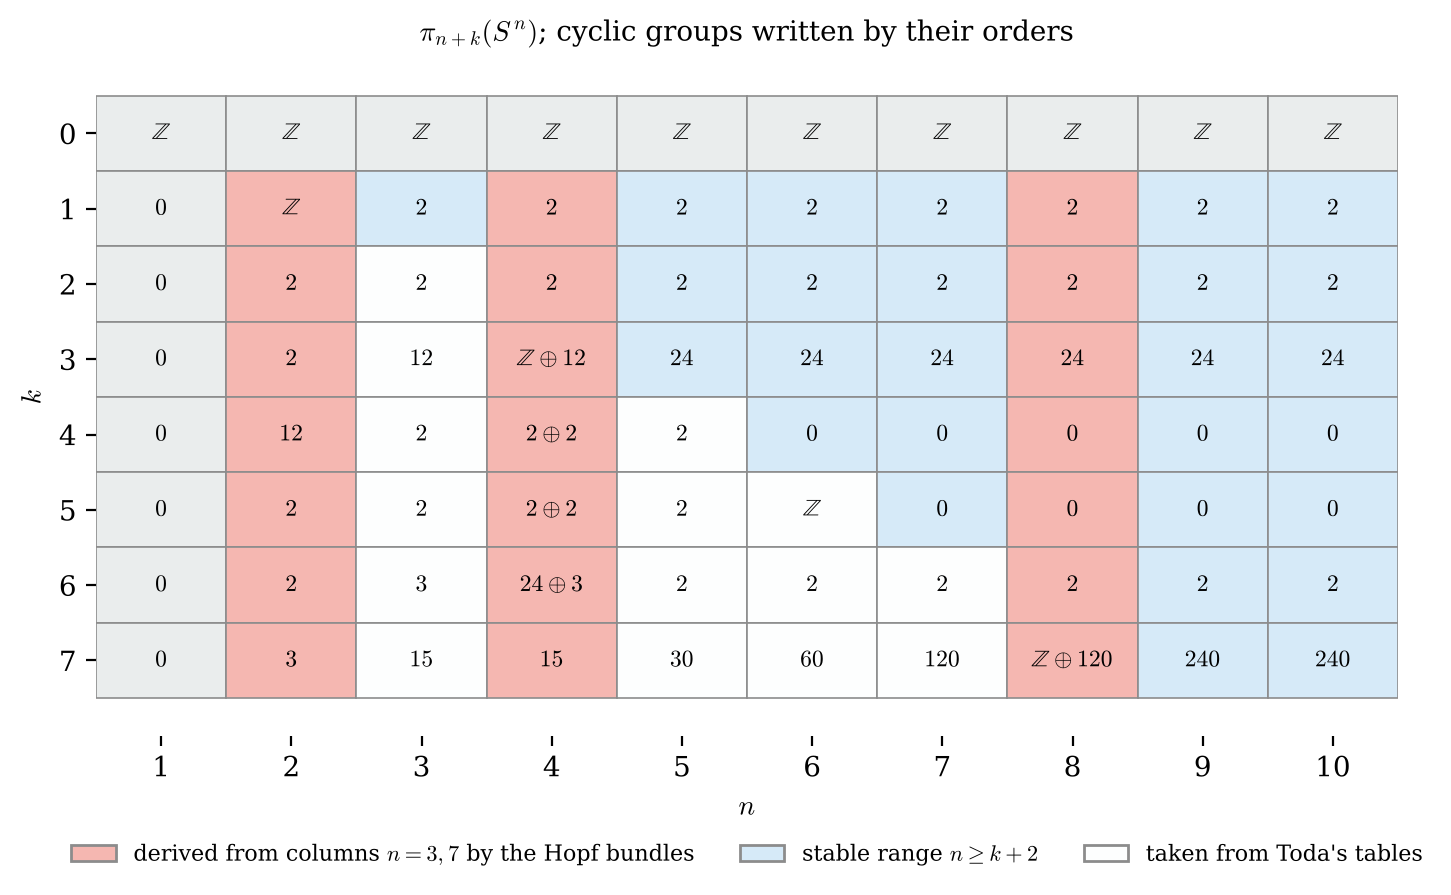
\includegraphics[width=0.95\textwidth]{fig_table.png}
\caption{The table of $\pi_{n+k}(S^n)$. Dark cells are derived from the columns $n=3$ and $n=7$ by the Hopf bundles (Theorem~\ref{thm:C}); light cells lie in the stable range $n\ge k+2$ (Theorem~\ref{thm:freudenthal}); white cells are taken from Toda's tables.}
\label{fig:table}
\end{figure}

\begin{example}\label{ex:derived}
Reading the table through Theorem~\ref{thm:C}:
\begin{enumerate}[label=\textup{(\alph*)}]
\item $\pi_4(S^2)\cong\pi_4(S^3)\cong\Z/2$, $\pi_5(S^2)\cong\pi_5(S^3)\cong\Z/2$, $\pi_6(S^2)\cong\pi_6(S^3)\cong\Z/12$.
\item $\pi_8(S^4)\cong\pi_8(S^7)\oplus\pi_7(S^3)\cong(\Z/2)^2$ and $\pi_9(S^4)\cong\pi_9(S^7)\oplus\pi_8(S^3)\cong(\Z/2)^2$.
\item $\pi_{10}(S^4)\cong\pi_{10}(S^7)\oplus\pi_9(S^3)\cong\Z/24\oplus\Z/3$.
\item $\pi_{i}(S^8)\cong\pi_{i-1}(S^7)$ for $8\le i\le14$, and $\pi_{15}(S^8)\cong\Z\oplus\Z/120$.
\end{enumerate}
In each case the summand $\pi_i(S^{2d-1})$ is the image of composition with the Hopf map, and the summand $\pi_{i-1}(S^{d-1})$ is the image of the suspension.
\end{example}

\subsection{Generators}\label{sec:generators}

In Toda's notation \cite{Tod62} the Hopf maps are $\eta_2=[h_\C]$, $\nu_4=[h_\Hq]$ and $\sigma_8=[h_\Oc]$, and $\eta_n$, $\nu_n$, $\sigma_n$ denote their iterated suspensions. The stable stems in degrees $1$, $3$ and $7$ are cyclic of orders $2$, $24$ and $240$, generated by $\eta$, $\nu$ and $\sigma$ \cite[Chapters~V and XIV]{Tod62}. Before suspension the Hopf maps have infinite order, since their Hopf invariant is $\pm1$ (Theorem~\ref{thm:B}); after suspension they have finite order and generate the image of the $J$-homomorphism in these degrees (Section~\ref{ch:stable}). For instance, $E^2\nu'=2\nu_5$ for the generator $\nu'$ of $\pi_6(S^3)\cong\Z/12$ \cite[Chapter~V]{Tod62}, so the summand $E\pi_6(S^3)$ of $\pi_7(S^4)$ maps onto the subgroup of index two of $\pi_8(S^5)\cong\Z/24$, and the summand $\Z\nu_4$ maps onto the whole group.
